\documentclass[11pt,a4paper]{article}
\usepackage[T1]{fontenc}
\usepackage[utf8]{inputenc}
\usepackage{lmodern}
\usepackage[a4paper,margin=25mm]{geometry}
\usepackage{microtype}
\usepackage{amsmath,amssymb}
\usepackage{booktabs,longtable,array}
\usepackage{enumitem}
\usepackage{url}
\usepackage[hidelinks]{hyperref}
\usepackage{tikz}
\usetikzlibrary{arrows.meta,positioning,calc}
\setlength{\parindent}{0pt}
\setlength{\parskip}{6pt}
\setlength{\emergencystretch}{2em}
\renewcommand{\arraystretch}{1.2}
\setlist{nosep,leftmargin=*}
\pagestyle{plain}
\raggedbottom
\date{}
\hypersetup{pdfauthor={Hariprasad},pdftitle={AIOps Capstone Project - MathStudio}}
\begin{document}
\begin{titlepage}
\begin{center}
{\large Hariprasad}\\[4pt]
{\large Roll Number: DA24B005}\\[20pt]
{\LARGE\bfseries AIOps Capstone Project -- MathStudio}\\[8pt]
{\large Local Mathematics Assistant}\\[18pt]
\end{center}
\begin{center}
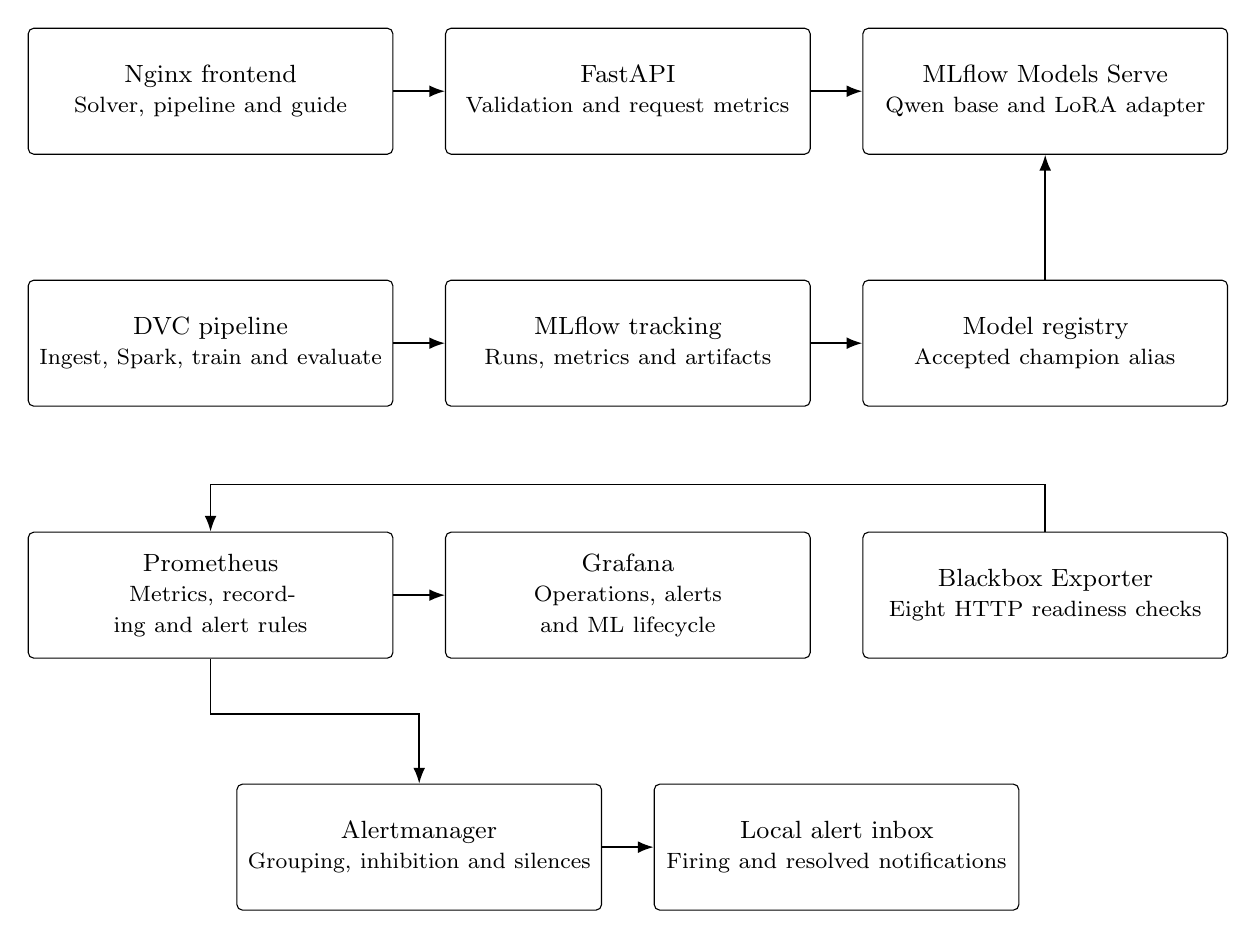
\begin{tikzpicture}[
 box/.style={draw,rounded corners=2pt,align=center,text width=43.5mm,minimum height=16mm,inner sep=4pt,font=\small},
 flow/.style={-{Latex[length=2mm]},semithick}]
\node[box] (ui) at (0,0) {Nginx frontend\\\footnotesize Solver, pipeline and guide};
\node[box] (api) at (5.3,0) {FastAPI\\\footnotesize Validation and request metrics};
\node[box] (serve) at (10.6,0) {MLflow Models Serve\\\footnotesize Qwen base and LoRA adapter};
\draw[flow] (ui.east)--(api.west);
\draw[flow] (api.east)--(serve.west);
\node[box] (dvc) at (0,-3.2) {DVC pipeline\\\footnotesize Ingest, Spark, train and evaluate};
\node[box] (track) at (5.3,-3.2) {MLflow tracking\\\footnotesize Runs, metrics and artifacts};
\node[box] (registry) at (10.6,-3.2) {Model registry\\\footnotesize Accepted champion alias};
\draw[flow] (dvc.east)--(track.west);
\draw[flow] (track.east)--(registry.west);
\draw[flow] (registry.north)--(serve.south);
\node[box] (prom) at (0,-6.4) {Prometheus\\\footnotesize Metrics, recording and alert rules};
\node[box] (graf) at (5.3,-6.4) {Grafana\\\footnotesize Operations, alerts and ML lifecycle};
\node[box] (probe) at (10.6,-6.4) {Blackbox Exporter\\\footnotesize Eight HTTP readiness checks};
\draw[flow] (prom.east)--(graf.west);
\draw[flow] (probe.north)--++(0,0.6)-|(prom.north);
\node[box] (am) at (2.65,-9.6) {Alertmanager\\\footnotesize Grouping, inhibition and silences};
\node[box] (inbox) at (7.95,-9.6) {Local alert inbox\\\footnotesize Firing and resolved notifications};
\draw[flow] (prom.south)--++(0,-0.7)-|(am.north);
\draw[flow] (am.east)--(inbox.west);
\end{tikzpicture}
\end{center}
The solver sends a question to FastAPI, which calls the registered Qwen model through MLflow Models Serve. The DVC pipeline handles data preparation, training and evaluation. MLflow keeps the runs and model artifacts, while Prometheus, Grafana and Alertmanager track service health and alert delivery.
\end{titlepage}
\setcounter{page}{2}
\section*{Architecture}
\subsection*{Runtime path}
The workspace and pipeline console are static frontend screens. FastAPI defines a narrow REST boundary. Model serving is a separate service using the registered executable pyfunc model. The web process does not load a second copy of the model. Prometheus scrapes API, pipeline, model-process, Grafana and its own operational metrics. Grafana provides service, incident and ML lifecycle dashboards. Prometheus evaluates seventeen alert rules and six recording rules. Blackbox probes check eight HTTP endpoints. Alertmanager groups, deduplicates, inhibits and routes firing/resolved notifications to the persistent local inbox. Seven metrics targets and the HTTP probes are scraped every fifteen seconds. The stack has nine Compose services with loopback-only host ports. See the monitoring runbook for thresholds and incident response.

\subsection*{Build and experiment path}
Environment inspection is an independent stage. EDA and Spark both depend on ingestion. Base evaluation depends on the held-out split; adapter evaluation additionally depends on training. The generation gate uses the saved adapter and predeclared prompts. Registration requires both adapter evaluation and acceptance evidence. The parent runner executes inspection, EDA and the requested dependency closure.

DVC caches datasets, split files, model directories and measured reports. MLflow stores training-step metrics, stage timings, run outcomes, output hashes, reports, source snapshots, dependency versions and registry decisions. The local submission archive includes the DVC object store; a separate restoration command reconstructs MLflow registration for a different folder path.

See High-level design for rationale, Low-level design for exact interfaces, and Operator runbook for execution and rollback.

\clearpage
\section*{High-Level Design}
\subsection*{Problem and intended outcome}
Students practising mathematics need a simple way to request a worked explanation without sending questions to a hosted inference API. MathStudio serves a locally fine-tuned small language model through a solver. Operators can inspect the complete data and model lifecycle in a separate pipeline console. I used a CPU setup so the complete workflow can run on one machine.

Success means the user can submit a question, receive a generated answer, recover from invalid input, and inspect measured operational evidence. Engineering acceptance requires passing automated tests, a completed reproducible DVC graph, an acceptance decision bound to the actual adapter weights, a registered executable MLflow model, and working monitoring exporters. Model smoke acceptance requires at least 80\% on the five predeclared cases. This small suite is not a broad mathematics benchmark.

\subsection*{Functional blocks and boundaries}
The independent Nginx frontend contains HTML, CSS and JavaScript. It calls only configurable REST URLs. It never reads model files, imports Python, or connects directly to a database. Nginx provides a same-origin reverse proxy; \texttt{frontend/\allowbreak{}config.\allowbreak{}js} permits a separate API origin. FastAPI owns validation, response contracts, error translation and request instrumentation. \texttt{ModelService} isolates the inference transport from the API route functions.

The deployed inference engine is MLflow Models Serve on port 5002, loading the accepted registry alias \texttt{champion}. Its pyfunc wrapper loads the pinned Qwen base and the registered LoRA artifact. This makes the model an independently exposed inference service, rather than merely storing files in an experiment tracker. A lock serializes CPU inference. An optional lazy direct Transformers mode supports local development.

The operator runs the DVC DAG through \texttt{src.\allowbreak{}pipeline.\allowbreak{}run}. The runner takes a filesystem lock, creates a parent MLflow run, preserves source and dependency identities, and executes the declared stages. Each stage has a child experiment run, durable status, duration, output hashes and explicit exception reporting. A separate console reads these files through REST and links to the tool interfaces. The UI does not launch unrestricted shell commands.

\subsection*{Design choices and rationale}
\begingroup\small
\begin{longtable}{@{}>{\raggedright\arraybackslash}p{0.3333\dimexpr\textwidth-24pt\relax}>{\raggedright\arraybackslash}p{0.3333\dimexpr\textwidth-24pt\relax}>{\raggedright\arraybackslash}p{0.3333\dimexpr\textwidth-24pt\relax}@{}}
\toprule
\textbf{Choice} & \textbf{Rationale} & \textbf{Tradeoff} \\
\midrule
\endfirsthead
\textbf{Choice} & \textbf{Rationale} & \textbf{Tradeoff} \\
\midrule
\endhead
Qwen 2.5 0.5B with rank-8 LoRA & Fits local CPU resources; only 1,081,344 parameters are trained & Limited reasoning capability; answers require checking \\
Pinned model/data revisions & Establish immutable source identities & Initial setup needs public artifact downloads \\
Bounded 800-row ingestion & Makes a complete CPU experiment practical & The sample does not represent the entire NuminaMath corpus \\
Local Spark & Demonstrates distributed-style data transformations with bounded resources & Startup overhead is significant for a small dataset \\
Hash-based split by normalized question & Keeps question duplicates in one partition and supports reproducibility & Exact partition sizes vary from nominal 80/10/10 \\
Completion-only labels & Avoids optimizing the model to reproduce the prompt & Long prompts can mask every completion token; these are counted and excluded \\
DVC + MLflow & Separates artifact dependency/version control from experiment history/registry & Portable submissions must include the DVC object store and recreate absolute-path registry entries \\
Independent inference service & Separates REST orchestration from model loading & Adds one local service and a network boundary \\
SQLite and local files & Keeps the assignment self-contained & Single-machine demonstration, not a multi-host production database \\
Polling console every five seconds & Near real-time visibility with little operational complexity & State can be up to five seconds behind the pipeline \\
\bottomrule
\end{longtable}
\endgroup
\subsection*{Deployment and resource model}
Compose packages frontend, backend, model serving, MLflow tracking, Prometheus, Grafana, Alertmanager, Blackbox Exporter and a persistent alert inbox as nine services. Host ports bind to loopback. Monitoring uses 19090 and 13000 to coexist with the machine's other assignments. The model cache is mounted read-only into inference; only the selected base/adapter is loaded. Avoid running a second training process while the inference service is resident on a low-memory machine.

The source code is organized primarily around functions for data and training stages, with small objects at configuration and model-service boundaries. This supports replaceable inference transports and narrow tests. Request logs omit the question text. Detailed unexpected exceptions remain in operator logs while the user receives a stable error message.

\subsection*{Model decision and rollback}
Evaluation preserves raw completions and a SHA-256 hash of the adapter. The verifier recomputes case decisions and accuracy. Registration refuses mismatched base revisions or adapter weights, records a model version, and changes \texttt{champion} only for an accepted candidate. Failed candidates remain visible for review. For rollback, select a previously validated registry version and reset the alias with the MLflow client, then restart \texttt{model-\allowbreak{}serving}; see the operator runbook. No new version is silently described as accepted.

\clearpage
\section*{Low-Level Design and API Contract}
\subsection*{Services}
\begingroup\small
\begin{longtable}{@{}>{\raggedright\arraybackslash}p{0.3333\dimexpr\textwidth-24pt\relax}>{\raggedright\arraybackslash}p{0.3333\dimexpr\textwidth-24pt\relax}>{\raggedright\arraybackslash}p{0.3333\dimexpr\textwidth-24pt\relax}@{}}
\toprule
\textbf{Service} & \textbf{Host URL} & \textbf{Responsibility} \\
\midrule
\endfirsthead
\textbf{Service} & \textbf{Host URL} & \textbf{Responsibility} \\
\midrule
\endhead
Nginx frontend & \url{http://localhost:8080} & Workspace, pipeline console, guide and reverse proxy \\
FastAPI & \url{http://localhost:8000} & Input validation, REST orchestration, reports, request metrics \\
MLflow Models Serve & \url{http://localhost:5002} & Registered pyfunc inference \\
MLflow tracking & \url{http://localhost:5000} & Experiment history and model registry \\
Prometheus & \url{http://localhost:19090} & Exporter scrapes and alert rules \\
Grafana & \url{http://localhost:13000} & Service, alert and ML lifecycle dashboards \\
Alertmanager & \url{http://localhost:19093} & Alert routing, grouping and silences \\
Blackbox Exporter & Internal port 9115 & HTTP readiness probes \\
Alert inbox & \url{http://localhost:19199} & Local firing and resolved notification history \\
\bottomrule
\end{longtable}
\endgroup
\subsection*{Public application API}
\begingroup\small
\begin{longtable}{@{}>{\raggedright\arraybackslash}p{0.2500\dimexpr\textwidth-36pt\relax}>{\raggedright\arraybackslash}p{0.2500\dimexpr\textwidth-36pt\relax}>{\raggedright\arraybackslash}p{0.2500\dimexpr\textwidth-36pt\relax}>{\raggedright\arraybackslash}p{0.2500\dimexpr\textwidth-36pt\relax}@{}}
\toprule
\textbf{Endpoint} & \textbf{Input} & \textbf{Success response} & \textbf{Errors} \\
\midrule
\endfirsthead
\textbf{Endpoint} & \textbf{Input} & \textbf{Success response} & \textbf{Errors} \\
\midrule
\endhead
\texttt{GET /\allowbreak{}health} & none & \texttt{status}, \texttt{model\_\allowbreak{}loaded}, \texttt{configured}, \texttt{inference\_\allowbreak{}engine} & 200 indicates process liveness; model readiness is separate \\
\texttt{POST /\allowbreak{}v1/\allowbreak{}solve} & JSON \texttt{question}: string, trimmed, 1-8000 characters & \texttt{answer}: string; \texttt{latency\_\allowbreak{}seconds}: number; \texttt{model\_\allowbreak{}loaded}: boolean & 422 invalid or whitespace-only input; 503 inference unavailable; 500 unexpected inference failure \\
\texttt{GET /\allowbreak{}v1/\allowbreak{}pipeline/\allowbreak{}status} & none & \texttt{quality}, \texttt{splits}, \texttt{ingestion}, \texttt{evaluation}, \texttt{training}, \texttt{candidates}, \texttt{configured\_\allowbreak{}candidate}, \texttt{model\_\allowbreak{}loaded}, \texttt{model\_\allowbreak{}configured}, \texttt{pipeline}, \texttt{stages}, \texttt{registration}, \texttt{evidence\_\allowbreak{}source} & Missing/malformed optional reports are null; missing stage state is pending \\
\texttt{GET /\allowbreak{}v1/\allowbreak{}pipeline/\allowbreak{}logs} & none & \texttt{lines}: up to 80 strings from the bounded log tail & Missing logs produce an empty list \\
\texttt{GET /\allowbreak{}metrics} & none & Prometheus text exposition at this exact path & No redirect \\
\texttt{GET /\allowbreak{}docs}, \texttt{/\allowbreak{}openapi.\allowbreak{}json} & none & Interactive and machine-readable API contract & FastAPI defaults \\
\bottomrule
\end{longtable}
\endgroup
Example request:

\begin{quote}\small
\begin{verbatim}
{"question":"Solve 2x + 3 = 11 for x. Give only the final value."}
\end{verbatim}
\end{quote}
Example schema for a successful response (values are illustrative):

\begin{quote}\small
\begin{verbatim}
{"answer":"4","latency_seconds":0.9,"model_loaded":true}
\end{verbatim}
\end{quote}
Unavailable responses use \texttt{\{"detail":"The model service is starting or unavailable.\allowbreak{} Try again shortly.\allowbreak{}"\}}. Unexpected failures do not reveal server paths or exception text. The browser inserts generated text with \texttt{textContent}, then renders equations with local KaTeX assets in untrusted mode; model-provided HTML is never executed. Copy retains the original answer text.

\subsection*{MLflow inference interface}
\texttt{POST http:/\allowbreak{}/\allowbreak{}localhost:5002/\allowbreak{}invocations} consumes the registered signature:

\begin{quote}\small
\begin{verbatim}
{"dataframe_split":{"columns":["prompt"],"data":[["What is 7 multiplied by
8?"]]}}
\end{verbatim}
\end{quote}
It returns \texttt{\{"predictions":[".\allowbreak{}.\allowbreak{}.\allowbreak{}"]\}}. FastAPI converts one question to one row and extracts the first prediction. The transport has a 180-second timeout; the browser has a 190-second timeout. The wrapper applies the same requested-format chat instruction as the acceptance evaluator and direct development inference, tokenizes at most 2,048 input tokens, serializes access under a lock, uses greedy generation, and caps completions at 128 tokens. The base revision and adapter are registry artifacts, not browser-controlled parameters. A length-limit notice makes incomplete responses explicit. Restored deployments label submitted pipeline history and show fresh registry state separately.

\subsection*{Core modules and data contracts}
\texttt{Settings} is an immutable configuration object. \texttt{ModelService} owns local initialization or MLflow HTTP transport. \texttt{main.\allowbreak{}py} owns validation and HTTP behavior; its middleware measures success, validation failures, unavailable models and unexpected failures using bounded endpoint labels. \texttt{PipelineCollector} reads durable reports at scrape time, so metrics include command-line pipeline work.

\texttt{src.\allowbreak{}data.\allowbreak{}common} provides normalization, record identities, streaming JSONL I/O and file hashes. Spark trims and validates fields, normalizes whitespace, removes duplicates, sorts and emits records. Splitting uses a SHA-256 bucket of seed plus normalized question. Rows are sorted before writing, and the split report records counts and SHA-256 hashes. A normalized question cannot occur in two partitions.

The training adapter uses q/k/v/o attention projections, rank 8, alpha 16, dropout 0.05, float32, microbatch 1, accumulation 4, maximum length 256 and learning rate 0.00005. The seed is 42. Fully truncated completions are excluded and counted. Trainer callbacks send live numeric metrics to the stage MLflow run.

Stage state has \texttt{name}, \texttt{status}, \texttt{started\_\allowbreak{}at}, \texttt{run\_\allowbreak{}id}, \texttt{parent\_\allowbreak{}run\_\allowbreak{}id}, \texttt{command}, \texttt{git\_\allowbreak{}commit}, \texttt{git\_\allowbreak{}dirty}; completed/failed stages additionally have \texttt{seconds} and \texttt{finished\_\allowbreak{}at}. Completed stages record output hashes; failed stages record an error. Atomic replacement prevents partially written JSON. The parent runner uses \texttt{flock} to reject overlapping orchestrator runs.

\subsection*{Telemetry}
\begin{itemize}
\item API: request counts by endpoint/outcome and duration histograms; Python process/runtime metrics.
\item Pipeline: last stage duration and success gauge, Spark records/second and generation smoke accuracy.
\item Model process: prediction count, generation duration histogram, loaded state and process/runtime metrics on internal port 9101.
\item Infrastructure: scrape health plus Grafana and Prometheus self-metrics.
\end{itemize}
Availability alerts require one minute of sustained failure. Seventeen Prometheus alert rules cover service readiness, traffic-gated server errors and CPU latency, in-flight pressure, RSS, pipeline outcomes/stalls, acceptance and alerting health. Six recording rules normalize service indicators. Alertmanager groups, inhibits and routes firing/resolved notifications to a bounded persistent local inbox. A Watchdog verifies delivery; a controlled auto-expiring drill tests firing and resolution. No external notification destination is configured. See \texttt{monitoring/\allowbreak{}RUNBOOK.\allowbreak{}md} for exact thresholds and recovery commands.

\clearpage
\section*{Data}
The experiment uses a bounded snapshot of AI-MO/NuminaMath-1.5 at revision \texttt{1b05109f\allowbreak{}9e5c1ad0\allowbreak{}6c066351\allowbreak{}9502416c\allowbreak{}30b300f8}. Ingestion reads Parquet batches using range requests and stops after 800 rows, with a configured scan cap of 4,000. It does not download the entire corpus. The source link and upstream notices are in \texttt{THIRD\_\allowbreak{}PARTY\_\allowbreak{}NOTICES.\allowbreak{}md}.

The snapshot contains \texttt{problem}, \texttt{solution}, answer/validity metadata and source fields. The source-provided validity annotations identify 670 valid problems, 129 incomplete problems and one record containing multiple problems; solution annotations identify 737 valid, 61 incomplete, one NaN and one unsolved solution. All 800 sampled records are labeled \texttt{olympiads} and \texttt{synthetic=False} by the source. These descriptions apply to this bounded snapshot, not the whole dataset.

Spark trims fields, rejects null/empty problems and missing/too-short/too-long solutions, normalizes question whitespace/case for identity, removes exact normalized-question/solution duplicates, sorts the output and writes JSON. It retains 799 records. The split stage further deduplicates normalized questions regardless of their solution, leaving 798 rows: 642 training, 83 validation and 73 test. The split report records SHA-256 hashes; the live verification checks question-set disjointness.

The split uses seed 42 and a SHA-256 bucket of the normalized question. It avoids dependence on input row order and keeps duplicate question variants out of different partitions. Training also reports fully truncated examples whose response tokens cannot be supervised within 256 tokens; these are excluded rather than silently treated as usable training examples.

This pipeline's validity gate is structural. It does not discard every source record annotated incomplete or independently verify mathematical truth. The EDA and 25-row review preserve those annotations and warnings for audit. The first-row sample and its Olympiad source concentration limit representativeness, and maximum token length favors short visible completions. Expert curation, validity-based ablations and a broader unseen correctness benchmark are appropriate next experiments.

Raw stage reports, EDA distributions, the sample review, split hashes and measured throughput are DVC outputs and are copied to \texttt{reports/\allowbreak{}evidence/\allowbreak{}} for submission review.

\clearpage
\section*{Model}
\subsection*{Selected model and purpose}
Qwen/Qwen2.5-0.5B-Instruct at revision \texttt{7ae55760\allowbreak{}4adf67be\allowbreak{}50417f59\allowbreak{}c2c2f167\allowbreak{}def9a775}, with a locally trained rank-8 LoRA adapter. The intended application is single-user mathematics practice and an AIOps lifecycle demonstration on a CPU. The model provides generated explanations that users should check.

\subsection*{Training and lineage}
Training uses the bounded NuminaMath snapshot described in the data section. Only attention q/k/v/o LoRA parameters are updated. Prompt labels are masked, truncated completions are counted, and one epoch uses float32, batch size 1, accumulation 4, learning rate 0.00005 and seed 42. The evaluation report contains measured counts, loss and duration. DVC records artifacts and dependencies; MLflow records live training metrics, source/environment identity and the registered model version.

\subsection*{Evaluation}
Base and adapter completion loss are compared on the same 73-row held-out test partition. A separate five-question generated-answer smoke suite declares its expected patterns before execution and uses an 80\% threshold. The report retains every answer and the adapter hash. Registry promotion verifies that identity and recomputes the saved case decisions. These checks are bounded functionality evidence; neither low loss nor five successful simple answers proves general mathematical correctness.

\subsection*{Serving behavior}
The accepted \texttt{champion} alias is loaded by MLflow Models Serve. FastAPI validates questions and calls the registered dataframe signature. Generation is greedy, CPU access is serialized, inputs are limited to 2,048 tokens after request validation, and outputs to 128 new tokens. The UI supports questions of at most 8,000 characters. The model has no calculator, symbolic solver or retrieval tool attached.

\subsection*{Limits}
Long or complex reasoning can fail, incomplete reference solutions are present in the snapshot, and source sampling is concentrated in Olympiad problems. Users should verify numeric results and reasoning. There is no multi-user capacity guarantee or broad independent mathematics benchmark in this submission. The upstream base model retains its own notices; see \texttt{THIRD\_\allowbreak{}PARTY\_\allowbreak{}NOTICES.\allowbreak{}md}.

\clearpage
\section*{Evaluation and Training Evidence}
\subsection*{Training setup}
The current run uses Qwen/Qwen2.5-0.5B-Instruct at revision \texttt{7ae55760\allowbreak{}4adf67be\allowbreak{}50417f59\allowbreak{}c2c2f167\allowbreak{}def9a775}. The source dataset is AI-MO/NuminaMath-1.5 at revision \texttt{1b05109f\allowbreak{}9e5c1ad0\allowbreak{}6c066351\allowbreak{}9502416c\allowbreak{}30b300f8}. The bounded ingest writes 800 records; Spark retains 799. Question-level deduplication leaves 798 split rows: 642 train, 83 validation and 73 test. The validation partition is reserved.

Training uses rank 8, alpha 16, dropout 0.05, q/k/v/o attention projections, float32 CPU execution, microbatch 1, gradient accumulation 4, sequence length 256, learning rate 0.00005 and seed 42. 634 examples have visible completion labels; 8 fully truncated completions are excluded. The adapter has 1,081,344 trainable parameters. One epoch took 1642.0 seconds.

\begingroup\small
\begin{longtable}{@{}>{\raggedright\arraybackslash}p{0.2500\dimexpr\textwidth-36pt\relax}>{\raggedright\arraybackslash}p{0.2500\dimexpr\textwidth-36pt\relax}>{\raggedright\arraybackslash}p{0.2500\dimexpr\textwidth-36pt\relax}>{\raggedright\arraybackslash}p{0.2500\dimexpr\textwidth-36pt\relax}@{}}
\toprule
\textbf{Candidate} & \textbf{Held-out rows scored} & \textbf{Mean completion cross-entropy} & \textbf{Evaluation duration} \\
\midrule
\endfirsthead
\textbf{Candidate} & \textbf{Held-out rows scored} & \textbf{Mean completion cross-entropy} & \textbf{Evaluation duration} \\
\midrule
\endhead
Qwen base & 73 & 1.4872 & 86.2 s \\
Qwen LoRA & 73 & 1.3505 & 92.2 s \\
\bottomrule
\end{longtable}
\endgroup
The adapter lowers held-out completion loss by 9.2\%. This measures fit to reference completions and does not itself establish correct mathematics. Both models are evaluated sequentially on the same deterministic test split with prompt labels masked and a maximum length of 256.

\subsection*{Generated-answer smoke acceptance}
\texttt{configs/\allowbreak{}generation\_\allowbreak{}benchmark.\allowbreak{}json} contains five predeclared prompts spanning algebra, arithmetic, fractions, geometry and percentages. Greedy CPU generation saves every raw completion and tests the declared answer patterns. The verifier recomputes every decision and rejects inconsistent accuracy, statuses, duplicated cases and invalid thresholds.

The model returned \textbf{5/5 (100\%)}, against a threshold of 80\%, in 3.70 seconds. The score covers these five questions. It is separate from the held-out completion-loss measurement.

\begingroup\small
\begin{longtable}{@{}>{\raggedright\arraybackslash}p{0.3333\dimexpr\textwidth-24pt\relax}>{\raggedright\arraybackslash}p{0.3333\dimexpr\textwidth-24pt\relax}>{\raggedright\arraybackslash}p{0.3333\dimexpr\textwidth-24pt\relax}@{}}
\toprule
\textbf{Case} & \textbf{Passed} & \textbf{Raw generated answer} \\
\midrule
\endfirsthead
\textbf{Case} & \textbf{Passed} & \textbf{Raw generated answer} \\
\midrule
\endhead
ALG-01 & True & $x = 4$ \\
ARITH-01 & True & 56 \\
FRAC-01 & True & $\frac{7}{8}$ \\
GEOM-01 & True & $36$ \\
PCT-01 & True & 30 \\
\bottomrule
\end{longtable}
\endgroup
\subsection*{Resource, lineage and deployment evidence}
The three-step CPU preflight measured 2.109 seconds/microstep and 3.51 GiB process RSS, below the declared six-GiB benchmark gate. This is the benchmark's observed RSS, not a claimed peak for the entire training epoch. Spark cleaning measured 75.4 records/second including its measured transformation/write work.

The completed pipeline parent run is \texttt{32e03182\allowbreak{}71474a03\allowbreak{}b44ccfd0\allowbreak{}e98f759c}. Every stage records its own run ID, duration, command, Git commit/dirty state and output hashes. Training-step loss is logged live. A source snapshot and dependency freeze preserve the uncommitted training context; the final submission manifest identifies the delivered source.

The accepted model is registered as \texttt{local-\allowbreak{}math-\allowbreak{}assistant-\allowbreak{}qwen-\allowbreak{}cpu-\allowbreak{}v2} and served through the \texttt{champion} alias. The selected adapter SHA-256 is \texttt{250f3948\allowbreak{}52745ef1\allowbreak{}6ea716c7\allowbreak{}d0937a5b\allowbreak{}3ec78640\allowbreak{}28e79eb5\allowbreak{}d25d9bd4\allowbreak{}999d9267}. Registration checks that the persisted generation report names that exact adapter and base revision before moving \texttt{champion}. MLflow Models Serve loads that executable registry artifact, and the live runtime checks exercise the actual web inference path.

\clearpage
\section*{Results and Outputs}
I checked the application at the API, pipeline and browser levels. The checks below use the project environment and the running local services. The JUnit output is in \texttt{reports/\allowbreak{}test-\allowbreak{}results.\allowbreak{}xml}; the live check reports and screenshots are kept in \texttt{reports/\allowbreak{}evidence/\allowbreak{}} and \texttt{docs/\allowbreak{}screenshots/\allowbreak{}}.

\begingroup\small
\begin{longtable}{@{}>{\raggedright\arraybackslash}p{0.5000\dimexpr\textwidth-12pt\relax}>{\raggedright\arraybackslash}p{0.5000\dimexpr\textwidth-12pt\relax}@{}}
\toprule
\textbf{Check} & \textbf{Measured result} \\
\midrule
\endfirsthead
\textbf{Check} & \textbf{Measured result} \\
\midrule
\endhead
Unit and contract tests & 58 passed; no failures or skipped cases \\
Application and live inference checks & 10 passed \\
Monitoring checks & 15 passed, including all dashboard queries and real alert delivery \\
Alert-rule scenarios & 9 passed \\
Recording-rule scenarios & 2 passed \\
Browser checks & 9 passed, including input feedback, example questions and mobile layout \\
Selected-model pipeline & All 11 stages completed \\
CPU resource benchmark & 2.109 seconds per microstep; 3.51 GiB process RSS \\
Spark cleaning & 799 of 800 records retained; 75.4 records per second \\
Generation smoke suite & 5 of 5 declared questions passed \\
Running stack & 9 services, 15 scrape targets, 8 HTTP probes and 3 dashboards \\
MLprojects test entry point & Passed in the project environment \\
\bottomrule
\end{longtable}
\endgroup
\subsection*{Application outputs}
These are the answers returned through the solver. FastAPI passes each question to MLflow Models Serve, then the browser renders the returned answer.

\begingroup\small
\begin{longtable}{@{}>{\raggedright\arraybackslash}p{0.5000\dimexpr\textwidth-12pt\relax}>{\raggedright\arraybackslash}p{0.5000\dimexpr\textwidth-12pt\relax}@{}}
\toprule
\textbf{Question} & \textbf{Returned answer} \\
\midrule
\endfirsthead
\textbf{Question} & \textbf{Returned answer} \\
\midrule
\endhead
Solve $2x+3=11$ for $x$. Give only the final value. & $x=4$ \\
What is 7 multiplied by 8? & $56$ \\
What is $3/4+1/8$? Give only the simplified fraction. & $\frac{7}{8}$ \\
Area of a rectangle with length 9 and width 4. & $36$ \\
What is 15 percent of 200? & $30$ \\
\bottomrule
\end{longtable}
\endgroup
The five-question outputs above are saved in the generation report. The separate HTTP checks also returned the correct algebra and fraction answers through Nginx, FastAPI and the model-serving endpoint.

\subsection*{Verification output}
The unit-test command returned:

\begin{quote}\small
\begin{verbatim}
58 passed
\end{verbatim}
\end{quote}
The running-service checks returned:

\begin{quote}\small
\begin{verbatim}
Application checks: 10 passed, 0 failed
Monitoring checks: 15 passed, 0 failed
HTTP readiness: 8 / 8 endpoints ready
Scrape inventory: 15 / 15 targets up
\end{verbatim}
\end{quote}
The alert-delivery check returned:

\begin{quote}\small
\begin{verbatim}
PASS: Recent real Watchdog notification delivered
PASS: Controlled alert reached inbox as firing
PASS: Controlled alert reached inbox as resolved
\end{verbatim}
\end{quote}
The drill enabled a temporary metric, waited for Prometheus to fire the rule, and checked that Alertmanager delivered it to the local inbox. Disabling the metric produced a resolved notification. The application stayed available during the check.

\subsection*{Integration checks}
The API handled empty questions, invalid input, unavailable inference and unexpected errors with the expected response codes. Generated text was rendered safely in the browser. The mobile check used a 390-pixel viewport and found no horizontal overflow.

A pipeline diagnostic deliberately returned an error so failure tracking could be checked. During integration, an MLprojects interpreter mismatch, interrupted evaluation and a list-shaped EDA logging issue were corrected and the checks were rerun. The saved training epoch was reused when evaluation resumed. Formatting checks preserved the training code's syntax tree, and DVC metadata was refreshed without repeating the same computation. Failed runs remain in the experiment history.

The live checks also caught a stale backend address in Nginx after container recreation. The proxy now uses Docker DNS, and the API readiness probe goes through that proxy. The rerun passed both inference questions. Monitoring checks cover the running dashboards, rule evaluation, Watchdog delivery and the firing/resolved route.

\end{document}
